% Manuscript for the Physiological Measurement focus collection
% "Detection of Neglected Tropical Diseases from the Cardiac Signals".
% Every number comes from numbers.tex, every table from tables/, every figure from figures/;
% all three are generated by paper/make_assets.py from the saved experiment results.
% Build: bash paper/build.sh
\documentclass{iopjournal}
\usepackage{amsmath}
\usepackage{graphicx}
\usepackage[round,authoryear]{natbib}
\usepackage{tikz}
\usetikzlibrary{arrows.meta,positioning}
% generated by paper/make_assets.py -- do not edit
\newcommand{\nAll}{366,185}
\newcommand{\nTrain}{292,885}
\newcommand{\nTest}{73,300}
\newcommand{\nTestPos}{1,662}
\newcommand{\testPrev}{2.27}
\newcommand{\nCodeShort}{204,522}
\newcommand{\nCodeLong}{131,734}
\newcommand{\nCodeShortPos}{6,236}
\newcommand{\nCodeLongPos}{317}
\newcommand{\nCodePos}{6,559}
\newcommand{\prevShort}{3.05}
\newcommand{\prevLong}{0.24}
\newcommand{\prevRatio}{12.7}
\newcommand{\shareCodePosShort}{95.1}
\newcommand{\shareAllShort}{56}
\newcommand{\nSsevenPos}{1,259}
\newcommand{\nStenPos}{77}
\newcommand{\nSseven}{40,867}
\newcommand{\nSten}{26,435}
\newcommand{\nStenPlusPos}{240}
\newcommand{\durOnlyB}{0.677}
\newcommand{\durOnlyA}{0.647}
\newcommand{\rowZeroA}{0.412}
\newcommand{\rowZeroAauc}{0.847}
\newcommand{\rowZeroSseven}{0.377}
\newcommand{\rowZeroSsevenAuc}{0.807}
\newcommand{\rowZeroGap}{$+0.30$}
\newcommand{\bzA}{0.436}
\newcommand{\bzAsd}{0.010}
\newcommand{\bzAauc}{0.829}
\newcommand{\bzBauc}{0.830}
\newcommand{\bzSseven}{0.384}
\newcommand{\bzSsevenSd}{0.017}
\newcommand{\bzSsevenAuc}{0.787}
\newcommand{\bzStenAuc}{0.695}
\newcommand{\bzStenPlusAuc}{0.779}
\newcommand{\bzEnsA}{0.452}
\newcommand{\bzEnsSseven}{0.404}
\newcommand{\bzEnsSsevenAuc}{0.801}
\newcommand{\bzGap}{$+0.17$}
\newcommand{\bzNegShort}{0.57}
\newcommand{\bzNegLong}{0.40}
\newcommand{\fullAuc}{0.791}
\newcommand{\fullA}{0.427}
\newcommand{\fullSsevenAuc}{0.751}
\newcommand{\aucInflation}{0.043}
\newcommand{\ladderGainA}{0.023}
\newcommand{\ptbRowFour}{0.24}
\newcommand{\ptbRowFive}{0.01}
\newcommand{\ptbRowFiveB}{0.07}
\newcommand{\lrMidSseven}{0.381}
\newcommand{\lrLowSseven}{0.362}
\newcommand{\lrMidA}{0.423}
\newcommand{\lrLowA}{0.404}
\newcommand{\bestEpHigh}{1.7}
\newcommand{\bestEpMid}{2.7}
\newcommand{\bestEpLow}{6.7}
\newcommand{\mOneA}{0.401}
\newcommand{\mOneSseven}{0.382}
\newcommand{\mOneGap}{$+0.04$}
\newcommand{\mOneStenPlusAuc}{0.817}
\newcommand{\wOneA}{0.428}
\newcommand{\wOneSseven}{0.380}
\newcommand{\wOneGap}{$+0.10$}
\newcommand{\wOneSsevenAuc}{0.795}
\newcommand{\wOneStenPlusAuc}{0.835}
\newcommand{\mwA}{0.403}
\newcommand{\mwSseven}{0.375}
\newcommand{\mwSsevenSd}{0.011}
\newcommand{\mwSsevenAuc}{0.795}
\newcommand{\mwStenAuc}{0.773}
\newcommand{\mwStenPlusAuc}{0.841}
\newcommand{\mwStenPlus}{0.479}
\newcommand{\bzStenPlus}{0.462}
\newcommand{\mwGap}{$+0.01$}
\newcommand{\mOneSsevenSd}{0.003}
\newcommand{\wOneSsevenSd}{0.004}
\newcommand{\ensGainSseven}{0.020}
\newcommand{\mOneDSseven}{$-0.002$}
\newcommand{\mOneDSsevenSe}{0.005}
\newcommand{\wOneDSseven}{$-0.004$}
\newcommand{\wOneDSsevenSe}{0.004}
\newcommand{\wOneDSsevenAuc}{$+0.008$}
\newcommand{\wOneDSsevenAucSe}{0.002}
\newcommand{\frozenDSseven}{$-0.041$}
\newcommand{\mwDSseven}{$-0.009$}
\newcommand{\mwDSsevenSe}{0.005}
\newcommand{\mwDSsevenAuc}{$+0.008$}
\newcommand{\mwDSsevenAucSe}{0.003}
\newcommand{\mwDStenPlusAuc}{$+0.062$}
\newcommand{\mwDStenPlusAucSe}{0.011}
\newcommand{\wOneDStenPlusAuc}{$+0.056$}
\newcommand{\wOneDStenPlusAucSe}{0.010}
\newcommand{\mOneDStenPlusAuc}{$+0.037$}
\newcommand{\mOneDStenPlusAucSe}{0.009}
\newcommand{\mwEnsSseven}{0.396}
\newcommand{\mwEnsStenPlusAuc}{0.854}
\newcommand{\bzEnsStenPlusAuc}{0.801}
\newcommand{\frozenSseven}{0.343}
\newcommand{\frozenSsevenAuc}{0.775}
\newcommand{\frozenStenPlusAuc}{0.797}
\newcommand{\halfSseven}{0.370}
\newcommand{\halfSsevenAuc}{0.798}
\newcommand{\ftGainSseven}{0.032}
\newcommand{\bzSsevenC}{0.382}
\newcommand{\mwSsevenC}{0.376}

% generated by paper/make_assets.py -- do not edit
\newcommand{\rThreeBzA}{0.427}
\newcommand{\rThreeBzSseven}{0.385}
\newcommand{\rThreeBzSsevenAuc}{0.788}
\newcommand{\rThreeBzStenPlusAuc}{0.781}
\newcommand{\rThreeBzEnsSseven}{0.395}
\newcommand{\rThreeBzEnsStenPlusAuc}{0.809}
\newcommand{\rThreeBzGap}{$+0.15$}
\newcommand{\rThreeBzSrcGap}{$-0.04$}
\newcommand{\rThreeWoneA}{0.422}
\newcommand{\rThreeWoneSseven}{0.383}
\newcommand{\rThreeWoneSsevenAuc}{0.794}
\newcommand{\rThreeWoneStenPlusAuc}{0.824}
\newcommand{\rThreeWoneEnsSseven}{0.388}
\newcommand{\rThreeWoneEnsStenPlusAuc}{0.834}
\newcommand{\rThreeWoneGap}{$+0.08$}
\newcommand{\rThreeWoneSrcGap}{$-0.02$}
\newcommand{\rThreeWoneDSseven}{$-0.002 \pm 0.005$}
\newcommand{\rThreeWoneDSsevenAuc}{$+0.006 \pm 0.002$}
\newcommand{\rThreeWoneDStenPlusAuc}{$+0.043 \pm 0.010$}
\newcommand{\rThreeWfiveA}{0.417}
\newcommand{\rThreeWfiveSseven}{0.375}
\newcommand{\rThreeWfiveSsevenAuc}{0.792}
\newcommand{\rThreeWfiveStenPlusAuc}{0.824}
\newcommand{\rThreeWfiveEnsSseven}{0.397}
\newcommand{\rThreeWfiveEnsStenPlusAuc}{0.837}
\newcommand{\rThreeWfiveGap}{$+0.08$}
\newcommand{\rThreeWfiveSrcGap}{$-0.02$}
\newcommand{\rThreeWfiveDSseven}{$-0.010 \pm 0.005$}
\newcommand{\rThreeWfiveDSsevenAuc}{$+0.004 \pm 0.002$}
\newcommand{\rThreeWfiveDStenPlusAuc}{$+0.043 \pm 0.010$}
\newcommand{\rThreeWoneRA}{0.425}
\newcommand{\rThreeWoneRSseven}{0.389}
\newcommand{\rThreeWoneRSsevenAuc}{0.797}
\newcommand{\rThreeWoneRStenPlusAuc}{0.827}
\newcommand{\rThreeWoneREnsSseven}{0.410}
\newcommand{\rThreeWoneREnsStenPlusAuc}{0.841}
\newcommand{\rThreeWoneRGap}{$+0.01$}
\newcommand{\rThreeWoneRSrcGap}{$-0.01$}
\newcommand{\rThreeWoneRDSseven}{$+0.004 \pm 0.005$}
\newcommand{\rThreeWoneRDSsevenAuc}{$+0.009 \pm 0.003$}
\newcommand{\rThreeWoneRDStenPlusAuc}{$+0.046 \pm 0.012$}
\newcommand{\rThreeWoneSA}{0.414}
\newcommand{\rThreeWoneSSseven}{0.384}
\newcommand{\rThreeWoneSSsevenAuc}{0.793}
\newcommand{\rThreeWoneSStenPlusAuc}{0.819}
\newcommand{\rThreeWoneSEnsSseven}{0.390}
\newcommand{\rThreeWoneSEnsStenPlusAuc}{0.839}
\newcommand{\rThreeWoneSGap}{$+0.07$}
\newcommand{\rThreeWoneSSrcGap}{$-0.01$}
\newcommand{\rThreeWoneSDSseven}{$-0.001 \pm 0.005$}
\newcommand{\rThreeWoneSDSsevenAuc}{$+0.005 \pm 0.003$}
\newcommand{\rThreeWoneSDStenPlusAuc}{$+0.038 \pm 0.011$}
\newcommand{\rThreeWoneTtaA}{0.422}
\newcommand{\rThreeWoneTtaSseven}{0.383}
\newcommand{\rThreeWoneTtaSsevenAuc}{0.794}
\newcommand{\rThreeWoneTtaStenPlusAuc}{0.822}
\newcommand{\rThreeWoneTtaEnsSseven}{0.388}
\newcommand{\rThreeWoneTtaEnsStenPlusAuc}{0.832}
\newcommand{\rThreeWoneTtaGap}{$+0.09$}
\newcommand{\rThreeWoneTtaSrcGap}{$-0.02$}
\newcommand{\rThreeWoneTtaDSseven}{$-0.002 \pm 0.005$}
\newcommand{\rThreeWoneTtaDSsevenAuc}{$+0.006 \pm 0.002$}
\newcommand{\rThreeWoneTtaDStenPlusAuc}{$+0.041 \pm 0.010$}
\newcommand{\rThreeQualifies}{W1, W1R, W1S, W1tta}
\newcommand{\rThreeValN}{29,250}
\newcommand{\rThreeValPos}{681}
\newcommand{\rThreeTrainN}{89,954}
\newcommand{\rThreeTrainPos}{5,847}
\newcommand{\rThreeValPrev}{2.33}
\newcommand{\rThreeWoneRVsWoneDSseven}{$+0.006 \pm 0.005$}
\newcommand{\rThreeWoneRVsWoneDSsevenAuc}{$+0.003 \pm 0.003$}
\newcommand{\rThreeWoneRVsWoneDStenPlusAuc}{$+0.003 \pm 0.007$}
\newcommand{\rThreeWoneRVsWoneDEnsStenPlusAuc}{$+0.007 \pm 0.007$}
\newcommand{\rThreeWoneRVsWoneDEnsSseven}{$+0.021 \pm 0.007$}
\newcommand{\rThreeWoneSVsWoneDSseven}{$+0.001 \pm 0.004$}
\newcommand{\rThreeWoneSVsWoneDSsevenAuc}{$-0.001 \pm 0.003$}
\newcommand{\rThreeWoneSVsWoneDStenPlusAuc}{$-0.005 \pm 0.008$}
\newcommand{\rThreeWoneSVsWoneDEnsStenPlusAuc}{$+0.005 \pm 0.009$}
\newcommand{\rThreeWoneSVsWoneDEnsSseven}{$+0.002 \pm 0.007$}
\newcommand{\rThreeWoneTtaVsWoneDSseven}{$+0.000 \pm 0.000$}
\newcommand{\rThreeWoneTtaVsWoneDSsevenAuc}{$+0.000 \pm 0.000$}
\newcommand{\rThreeWoneTtaVsWoneDStenPlusAuc}{$-0.001 \pm 0.001$}
\newcommand{\rThreeWoneTtaVsWoneDEnsStenPlusAuc}{$-0.001 \pm 0.001$}
\newcommand{\rThreeWoneTtaVsWoneDEnsSseven}{$+0.000 \pm 0.000$}
\newcommand{\rThreeWfiveVsWoneDSseven}{$-0.008 \pm 0.002$}
\newcommand{\rThreeWfiveVsWoneDSsevenAuc}{$-0.002 \pm 0.001$}
\newcommand{\rThreeWfiveVsWoneDStenPlusAuc}{$+0.000 \pm 0.002$}
\newcommand{\rThreeWfiveVsWoneDEnsStenPlusAuc}{$+0.003 \pm 0.003$}
\newcommand{\rThreeWfiveVsWoneDEnsSseven}{$+0.009 \pm 0.004$}

\newcommand{\tpr}{TPR@5\%}
% The class prints template placeholders in the running head; name the target journal instead.
\fancyhead[L]{{\small \sf IOP Publishing}\hspace{5mm} {\it Physiol.\ Meas.}\ (manuscript)}
\fancyhead[R]{Nguyen {\it et al}\ }
\renewcommand{\articletype}[1]{{\vspace*{-8mm}\noindent \Large \sf Physiological Measurement}

\vspace{4mm}\noindent{\scriptsize \sf{\bfseries \MakeUppercase{#1}}}}

\begin{document}
\articletype{Paper}

\title{Record length is a label shortcut in the PhysioNet Challenge 2025 Chagas data: consequences for fine-tuning and evaluating an ECG foundation model}

% TODO(authors): confirm the author list, order, ORCIDs, affiliations and corresponding address.
% The list below is the team of the Challenge entry (Nguyen et al 2025) and is a placeholder.
\author{Kelvin Nguyen$^{1,*}$, Andy Smithwick$^1$, Maxwell Loetscher$^1$, Shadi Manafi$^1$, Zaniar Adarlan$^1$ and Saman Parvaneh$^1$}

\affil{$^1$Edwards Lifesciences, Irvine, CA, United States of America}

\affil{$^*$Author to whom any correspondence should be addressed.}

\email{kelvindinhnguyen@gmail.com}

\keywords{Chagas disease, electrocardiogram, foundation model, shortcut learning, dataset bias, PhysioNet Challenge, generalisation}

\begin{abstract}
\textit{Objective.} Models that detect Chagas disease from the 12-lead electrocardiogram (ECG) lost much of their internal performance on the hidden cohorts of the George B. Moody PhysioNet Challenge 2025. We sought a cause in the training data and tested its removal.
\textit{Approach.} We fine-tuned the ECG-FM foundation model on CODE-15\%, SaMi-Trop and PTB-XL with a patient-grouped held-out split, ran controlled ablations under pre-registered rules, and scored models within groups of equal record length.
\textit{Main results.} In CODE-15\%, \prevShort\% of 7.34 s recordings are labelled positive against \prevLong\% of 10.24 s recordings; length alone reaches an area under the receiver operating characteristic curve (AUROC) of \durOnlyB. Every model used this cue, inflating pooled AUROC by about \aucInflation; our ablation's apparent gain in the Challenge score (\rowZeroA{} to \bzA) vanished within length groups (\rowZeroSseven{} versus \bzSseven). Length-matched negatives with fixed 5 s windows removed the cue, changed the score within short recordings by less than 0.01, and raised AUROC on 10 s recordings from \bzStenPlusAuc{} to \mwStenPlusAuc. Averaging three seeds gained \ensGainSseven{} within length groups, more than any modelling change. With validation carved before the negative cap and scored within the shortcut-free format, a fixed-window model with a hard-negative ranking loss became the entry.
\textit{Significance.} Record length is a label shortcut in the Challenge training data that the hidden cohorts, all about 10 s long, do not share. Scoring within recording formats and removing the cue at the data level give a more faithful account of what an ECG model has learned.
\end{abstract}

\section{Introduction}
Chagas disease, caused by \textit{Trypanosoma cruzi}, affects millions of people in Latin America and is often silent for decades before it produces cardiomyopathy. Serological testing is the diagnostic standard but capacity is limited, so an inexpensive test that ranks people for serology is valuable. The 12-lead ECG is a natural candidate, because Chagas cardiomyopathy leaves conduction and rhythm abnormalities such as right bundle branch block and left anterior fascicular block \citep{jidling2023}.

The George B. Moody PhysioNet Challenge 2025 asked teams to rank ECGs by the probability of Chagas disease \citep{reyna2025,goldberger2000}. The score is the fraction of positive cases found among the 5\% of records with the highest predicted probability (\tpr). Training data came from three public sources with labels of very different quality: CODE-15\% with self-reported labels \citep{ribeiro2020}, SaMi-Trop with serologically confirmed positives \citep{cardoso2016}, and PTB-XL with presumed negatives \citep{wagner2020}. Models were scored on three hidden, serologically labelled Brazilian cohorts.

The outcome was sobering. The median score of the ranked teams fell from 0.279 on the hidden validation cohort to 0.236 and 0.100 on two of the test cohorts, and the best overall test score was 0.323 \citep{reyna2025}. Several teams reported internal scores that moved in the opposite direction to their hidden scores. One team reported a variant with a higher local score (0.827 against 0.627) and a lower hidden validation score (0.230 against 0.338) \citep{wang2025}. Our own entry, a frozen ECG-FM encoder \citep{mckeen2025} with a small classification head, scored 0.245 on the hidden test set, eighth of 40 ranked teams, and variants that scored higher internally scored far lower on the hidden data \citep{nguyen2025}.

When internal and external performance disagree this consistently, a likely explanation is that models learn a feature that predicts the label in the training data for reasons unrelated to the disease, a \emph{shortcut} \citep{geirhos2020}. In medical imaging, shortcuts have been traced to the hospital system and the acquisition device rather than the pathology \citep{zech2018,degrave2021}. The training data here invite the same problem. All SaMi-Trop records are positive and all PTB-XL records are negative, so the data source alone predicts the label. The winning team warned that the original sampling frequency and the mains interference frequency could act as such cues \citep{vansantvliet2025}.

This paper reports a shortcut that, to our knowledge, has not been described: within CODE-15\% itself, the \emph{length of the recording} predicts the Chagas label. We found it after a controlled ablation of our Challenge model produced gains that we could not explain. Our contributions are as follows.
\begin{enumerate}
\item We show that record length is strongly associated with the label in CODE-15\%, that a score based on length alone is far better than chance, and that every model we trained used it.
\item We show that pooled internal metrics are inflated by this cue, and that an eight-step ablation whose pooled score rose by \ladderGainA{} shows no improvement once records of equal length are compared.
\item We evaluate two remedies that act on the data rather than the model, length-matched negative sampling and fixed 5 s input windows, together with weight interpolation between the frozen and fine-tuned encoder and seed ensembling, and, under a validation protocol that cannot reward the shortcut, a hard-negative ranking loss, training without PTB-XL and overlapping-window inference.
\item We report what did not work, under decision rules fixed before each experiment, and give practical recommendations for evaluating models on these data.
\end{enumerate}

\section{Methods}
\subsection{Data and held-out split}
We used the public Challenge training data: CODE-15\% (400 Hz), SaMi-Trop (400 Hz) and PTB-XL (500 Hz), \nAll{} records in total after conversion to the Challenge format. CODE-15\% labels are self-reported, SaMi-Trop labels are serologically confirmed and all positive, and PTB-XL records are presumed negative because of their European origin \citep{reyna2025}.

CODE-15\% contains repeated examinations of the same patient, on average 1.48 per patient. A record-level split therefore leaks patients between partitions: in such a split of our data, 45.5\% of test examinations shared a patient with a training examination. We split by patient instead. Records were grouped by patient identifier (253,720 groups) and 20\% of the groups were held out, stratified by source and label. The held-out set has \nTest{} records and \nTestPos{} positives. We kept its natural prevalence of \testPrev\%, because \tpr{} is bounded above by 0.05 divided by the prevalence and so cannot be compared between sets of different prevalence. The remaining \nTrain{} records form the training split. Table \ref{tab:data} gives the composition. The length of every record was read from its WFDB header (number of samples divided by sampling frequency).

\begin{table}
\caption{Composition of the data by source and record length. Record length is the number of samples divided by the sampling frequency. The first group also contains the few records shorter than 5 s. Prevalence is over both splits.}
\centering
\small
\begin{tabular}{l l r r r r r}
\hline
 & & \multicolumn{2}{c}{Training split} & \multicolumn{2}{c}{Held-out split} & Prevalence \\
Source & Record length & Records & Positive & Records & Positive & (\%) \\
\hline
CODE-15\% & $<7.5$ s & 163,655 & 4,977 & 40,867 & 1,259 & 3.05 \\
 & 7.5--9.9 s & 5,226 & 6 & 1,273 & 0 & 0.09 \\
 & $\geq 9.9$ s & 105,299 & 240 & 26,435 & 77 & 0.24 \\
\hline
SaMi-Trop & $<7.5$ s & 564 & 564 & 147 & 147 & 100.00 \\
 & 7.5--9.9 s & 74 & 74 & 16 & 16 & 100.00 \\
 & $\geq 9.9$ s & 667 & 667 & 163 & 163 & 100.00 \\
\hline
PTB-XL & $\geq 9.9$ s & 17,400 & 0 & 4,399 & 0 & 0.00 \\
\hline
\end{tabular}

\label{tab:data}
\end{table}

\subsection{Metrics and statistics}
The primary metric is the Challenge score, \tpr. We also report the AUROC, which is independent of prevalence. Confidence intervals are 95\% percentile intervals from 1,000 bootstrap resamples of the test records \citep{efron1993}. To compare two configurations we used a paired bootstrap, resampling the same test records for both, and report the standard error (SE) of the difference. Unless stated otherwise, a configuration was trained with three random seeds and we report the mean and the standard deviation across seeds. A \emph{seed ensemble} is the mean of the predicted probabilities of the three models.

\subsection{Model and training}
Figure \ref{fig:pipeline} shows the pipeline. Leads were put in a fixed order and signals were resampled to 500 Hz with a polyphase filter. They were then band-pass filtered between 0.5 and 45 Hz (second-order Butterworth, zero phase) with notches at 50 and 60 Hz, and each lead was standardised to zero mean and unit variance over the whole record. In the baseline, the first 10 s of a record form one window; shorter records are zero-padded at the end and the padded positions are masked in the encoder's attention and in pooling.

The encoder is ECG-FM \citep{mckeen2025}, a convolutional front end followed by 12 transformer layers of width 768, for which we used the publicly released checkpoint. Following our Challenge entry \citep{nguyen2025}, the outputs of all 12 layers are combined with learnable softmax weights, averaged over time, and passed to a two-layer perceptron with 256 hidden units that outputs one logit.

Training has two stages \citep{vansantvliet2025,howard2018}. In stage 1 the encoder is frozen and only the layer weights and the head are trained for 2,000 optimiser steps at a learning rate of $2\times10^{-4}$. In stage 2 the 12 transformer layers are unfrozen, with the convolutional front end kept frozen as in the encoder's own fine-tuning recipe. The base learning rate is $2\times10^{-5}$, decayed by a factor of 0.85 per layer towards the input, with a cosine schedule and 5\% warm-up. We used a batch of 16 with gradient accumulation over four batches, 16-bit mixed precision, weight decay 0.01 and gradient clipping at 1.0. Ten per cent of the training patients were set aside for validation. The checkpoint with the best validation \tpr{} was kept and training stopped after three validations without improvement.

The loss is binary cross-entropy with a positive-class weight of 5. Targets are soft for the self-reported source: 0.8 and 0.2 for CODE-15\% positives and negatives, 1 for SaMi-Trop and 0 for PTB-XL \citep{vansantvliet2025}. For CODE-15\% patients with several examinations the target is $0.51\,y + 0.49\,n_{+}/n$, where $y$ is the record's label and $n_{+}/n$ the fraction of the patient's examinations labelled positive \citep{hong2025}. Positives were sampled five times as often as negatives. All positives were used, and negatives were subsampled so that a training run saw 100,000 records in total; section \ref{sec:res-train} reports the effect of this cap. Augmentations follow the top Challenge entries \citep{vansantvliet2025,hong2025}: resampling to and from another rate, random device-like filtering, mains interference at 50 or 60 Hz, baseline wander, Gaussian noise, amplitude scaling, time warping, random masking, and random cropping.

All training and inference ran through the unmodified Challenge entry scripts, so the code path is the one the organisers execute. Jobs ran on an NVIDIA Titan RTX with the memory allocator capped at 14.5 GiB to mimic the 16 GB graphics card of the Challenge environment. Peak memory in stage 2 was 4.1 GiB.

\begin{figure}
\centering
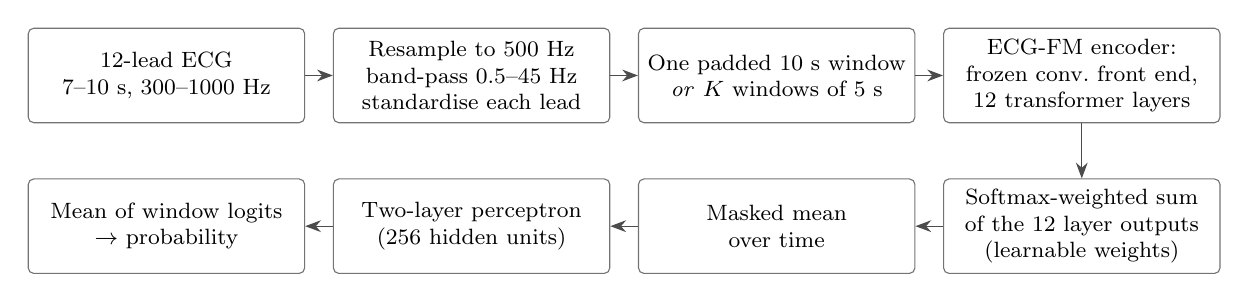
\begin{tikzpicture}[font=\footnotesize, node distance=6mm and 3.5mm,
  box/.style={draw=black!55, rounded corners=2pt, align=center, inner sep=3pt, minimum height=12mm, text width=33mm},
  arr/.style={-{Stealth[length=2mm]}, draw=black!70}]
\node[box] (ecg) {12-lead ECG\\7--10 s, 300--1000 Hz};
\node[box, right=of ecg] (pre) {Resample to 500 Hz\\band-pass 0.5--45 Hz\\standardise each lead};
\node[box, right=of pre] (win) {One padded 10 s window\\\emph{or} $K$ windows of 5 s};
\node[box, right=of win] (enc) {ECG-FM encoder:\\frozen conv.\ front end,\\12 transformer layers};
\node[box, below=7mm of enc] (agg) {Softmax-weighted sum\\of the 12 layer outputs\\(learnable weights)};
\node[box, left=of agg] (pool) {Masked mean\\over time};
\node[box, left=of pool] (head) {Two-layer perceptron\\(256 hidden units)};
\node[box, left=of head] (out) {Mean of window logits\\$\rightarrow$ probability};
\draw[arr] (ecg) -- (pre); \draw[arr] (pre) -- (win); \draw[arr] (win) -- (enc);
\draw[arr] (enc) -- (agg); \draw[arr] (agg) -- (pool); \draw[arr] (pool) -- (head); \draw[arr] (head) -- (out);
\end{tikzpicture}
\caption{The model. Stage 1 trains the layer weights and the perceptron with the encoder frozen; stage 2 also fine-tunes the 12 transformer layers with a learning rate that decays towards the input. The baseline uses one zero-padded 10 s window. The fixed-window variant uses $K=\lceil T/5\,\mathrm{s}\rceil$ evenly spaced 5 s windows of a record of length $T$ and averages their logits.}
\label{fig:pipeline}
\end{figure}

\subsection{Ablation ladder}
To attribute changes in performance we built the model in steps from our Challenge entry, each step adding one change to the previous one. Step 0 is the entry: frozen encoder, age and sex concatenated to the pooled feature, hard labels, and class-balanced sampling. Step 1 adds pipeline corrections (the padding mask, polyphase resampling, a vectorised band-pass filter) and the validation split with early stopping. Step 2 adds the soft labels and class weighting. Step 3 adds augmentation. Step 4 replaces the concatenation of age and sex with feature-wise modulation \citep{perez2018}. Step 5 adds stage-2 fine-tuning. Step 5b removes age and sex altogether, and step 5c lowers the upper band-pass frequency from 100 to 45 Hz. Steps 0 to 5c were trained once, on a fixed set of 100,000 training records. The final configuration (B0) is step 5c with the negative cap applied inside the training script, so that it can be trained from the full training split as the organisers would, and it was trained with three seeds. For B0 we also varied the stage-2 learning rate ($2\times10^{-5}$, $5\times10^{-6}$ and $10^{-6}$, the last being the rate used by the authors of ECG-FM), with three seeds each.

\subsection{Evaluation views}
We scored each model on several subsets of the held-out records.
\begin{description}
\item[A] All held-out records. Both the data source and the record length can be used as cues.
\item[B] CODE-15\% records only, which removes the source cue.
\item[S7] CODE-15\% records shorter than 7.5 s (\nSseven{} records, \nSsevenPos{} positives). Neither cue is available.
\item[S10] CODE-15\% records of at least 9.9 s (\nSten{} records, \nStenPos{} positives). Neither cue is available; this is the format of the hidden cohorts, but the number of positives is small.
\item[S10+] The negatives of S10 with all held-out positives of at least 9.9 s from CODE-15\% and SaMi-Trop (\nStenPlusPos{} positives). It has more power than S10 but reintroduces a source cue for the SaMi-Trop positives, so we treat it as secondary.
\item[C] View A after perturbations of the kind the organisers applied to the hidden data \citep{reyna2025}: resampling to and from 300, 500, 600 or 1000 Hz, a random device-like band-pass filter, Gaussian noise, baseline wander and mains interference.
\end{description}
Two diagnostics accompany every evaluation. The \emph{duration-only baseline} is the score of a predictor that outputs 1 for records shorter than 7.5 s and 0 otherwise. The \emph{length-cue gap} is the mean predicted probability of CODE-15\% negatives shorter than 7.5 s minus that of CODE-15\% negatives of at least 9.9 s. It is close to zero for a model that ignores record length.

\subsection{Removing the length cue}
\label{sec:methods-remedies}
\textit{Length-matched negative sampling.} When negatives are subsampled, they are drawn so that their distribution over three length groups (shorter than 7.5 s, 7.5 to 9.9 s, at least 9.9 s) equals that of the positives. Record length then carries no information about the label in the training or validation data. This is frequency matching of controls to cases on a confounder, and corresponds to the group-balancing remedy for spurious correlations \citep{idrissi2022,sagawa2020}. It costs nothing here, because two thirds of the negatives are discarded by the cap in any case.

\textit{Fixed 5 s windows.} ECG-FM was pretrained on 5 s segments \citep{mckeen2025}. With 5 s windows, no record of at least 5 s is padded, so the network cannot observe the record length. During training one random 5 s window is drawn per record per epoch. At validation and test time $K=\lceil T/5\,\mathrm{s}\rceil$ evenly spaced windows are evaluated and their logits averaged.

\textit{Weight interpolation.} A frozen encoder outperformed a fine-tuned one on hidden data for one Challenge team \citep{wang2025}, and fine-tuning can degrade out-of-distribution performance in general \citep{kumar2022}. To measure this we interpolated the weights of the stage-1 model ($\theta_1$, frozen encoder) and the stage-2 model ($\theta_2$) as $(1-\alpha)\theta_1+\alpha\theta_2$ \citep{wortsman2022} and scored $\alpha=0$, 0.5 and 1.

\textit{Seed ensembles.} Three models that differ only in the random seed are averaged \citep{lakshminarayanan2017}.

We trained three configurations with three seeds each, all derived from B0: matched negatives (M1), fixed windows (W1), and both (MW, scored at the three values of $\alpha$). Before the runs we fixed the rule for adopting a configuration: its mean \tpr{} on S7 must exceed that of B0 by more than the paired SE, or its S7 AUROC must be higher by more than 0.010 without a loss in S7 \tpr; in either case its S10+ AUROC must not fall by more than the SE. Views A, B and C were declared in advance not to be decision metrics, since they were expected to fall when the cue is removed.

\subsection{Round 3: a validation protocol that cannot see the shortcut}
\label{sec:meth-r3}
The experiments above selected checkpoints on the pooled validation \tpr, which the length cue inflates, and carved the validation set after the negative cap with the training seed, so that each seed validated on different records at the capped prevalence. For a final round we fixed the protocol. The validation set is drawn before the cap, at natural prevalence, from 10\% of the training patients stratified by source, label and length group, with a seed that does not change with the training seed and with PTB-XL grouped by patient as in the held-out split; it has \rThreeValN{} records and \rThreeValPos{} positives (\rThreeValPrev\%) and is identical for every run. Checkpoints are selected on the validation \tpr{} within 7.34 s CODE-15\% records. The negative cap is expressed as a training prevalence of 6.5\%, the value the 100,000-record cap gave on our split, so that it transfers to the organisers' larger training set. Seeds therefore differ only in initialisation and sampling, and ensemble members are selected on the same data.

Under this protocol we re-trained the baseline (B0) and the fixed-window model (W1) with three seeds, and tested three additions to W1 chosen for their expected value on 10 s recordings: a hard-negative ranking loss that acts directly on the top of the ranking \citep{hong2025} (W1R); training without PTB-XL, the only source that exists solely as negatives and is absent from the hidden data (W1S); and inference over overlapping 5 s windows every 2.5 s instead of $\lceil T/5\,\mathrm{s}\rceil$ disjoint ones (W1-TTA, no retraining). Two further W1 seeds measured the effect of a five-seed ensemble. Because the hidden cohorts are 10 s recordings, we fixed before the runs that the primary metric of this round is the S10+ AUROC with the S7 \tpr{} as a guard (not lower than B0 by more than one paired SE), that a variant replaces W1 only if it beats W1 on the primary metric by more than one SE, and that five members are used only if the five-seed ensemble beats the three-seed one by more than one SE. This change of primary view from round 2 was recorded as a decision with its reason before any result was seen.

\section{Results}
\subsection{Record length predicts the label in CODE-15\%}
CODE-15\% recordings come in two lengths, 7.34 s and 10.24 s (table \ref{tab:data}). Of the \nCodeShort{} records shorter than 7.5 s, \prevShort\% are labelled positive, against \prevLong\% of the \nCodeLong{} records of at least 9.9 s, a ratio of \prevRatio{} (figure \ref{fig:shortcut}(a)). As a result, \shareCodePosShort\% of the CODE-15\% positives are short records. About \shareAllShort\% of all training records are shorter than 7.5 s and so are zero-padded in a 10 s window. A predictor that uses only the record length reaches an AUROC of \durOnlyB{} on view B and \durOnlyA{} on view A.

\begin{figure}
\centering
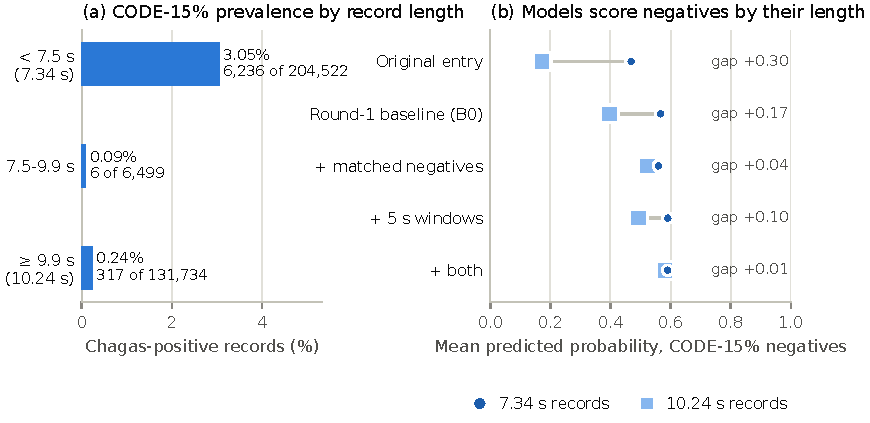
\includegraphics[width=\textwidth]{figures/fig_shortcut}
\caption{The length shortcut. (a) Prevalence of the Chagas label in CODE-15\% by record length, over all records. (b) Mean predicted probability of held-out CODE-15\% negatives, for 7.34 s records (circles) and 10.24 s records (squares). A model that ignores record length would give both groups the same mean. Values for configurations with several seeds are means over seeds.}
\label{fig:shortcut}
\end{figure}

\subsection{Every model used the cue, and pooled metrics were inflated}
All models, including the frozen-encoder Challenge entry, assigned higher probabilities to short records regardless of their label. For B0 the mean probability of held-out CODE-15\% negatives was \bzNegShort{} for short records and \bzNegLong{} for long ones, a length-cue gap of \bzGap{} (figure \ref{fig:shortcut}(b)); for the Challenge entry the gap was \rowZeroGap.

Scoring within one length group lowered the AUROC of every model by a similar amount (figure \ref{fig:inflation}, table \ref{tab:ladder}). For B0 the AUROC was \bzBauc{} on view B, \bzSsevenAuc{} within short records and \bzStenAuc{} within long records. The last value is close to the AUROCs of 0.68 and 0.59 that an earlier model obtained on REDS-II and ELSA-Brasil \citep{jidling2023}, two of the cohorts later used as hidden data in the Challenge. With only \nStenPos{} positives its confidence interval is wide, and it cannot rank models.

The consequence for the ablation is shown in table \ref{tab:ladder}. On view A the Challenge score rose from \rowZeroA{} for the entry to \bzA{} $\pm$ \bzAsd{} for B0. Within short records the same models scored \rowZeroSseven{} and \bzSseven{} $\pm$ \bzSsevenSd, a difference well inside the bootstrap SE of about 0.013, and the AUROC within short records was lower for B0 (\bzSsevenAuc) than for the entry (\rowZeroSsevenAuc). The gain measured on the pooled set was therefore not a gain in the detection of Chagas disease from ECG morphology.

\begin{figure}
\centering
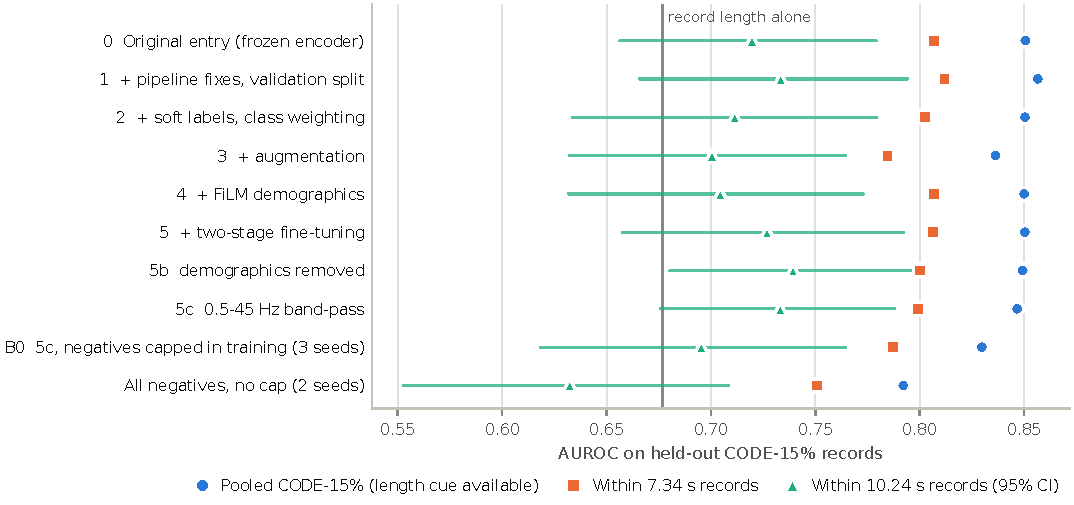
\includegraphics[width=0.95\textwidth]{figures/fig_inflation}
\caption{AUROC of each step of the ablation on held-out CODE-15\% records: pooled (view B), within 7.34 s records (S7) and within 10.24 s records (S10). The horizontal bars are 95\% bootstrap confidence intervals for S10, averaged over seeds where there are several. The vertical line is the AUROC of record length alone on view B.}
\label{fig:inflation}
\end{figure}

\begin{table}
\caption{The ablation ladder, scored on the pooled views and within record-length groups. The length-cue gap is the mean predicted probability of short CODE-15\% negatives minus that of long ones. Steps 0 to 5c are single runs; B0 and the uncapped run are means over seeds.}
\centering
\resizebox{\textwidth}{!}{\begin{tabular}{l c c c c c c c}
\hline
 & \multicolumn{2}{c}{Pooled (A)} & Pooled (B) & \multicolumn{2}{c}{Within 7.34 s (S7)} & 10.24 s (S10) & Length-cue \\
Configuration & TPR@5\% & AUROC & AUROC & TPR@5\% & AUROC & AUROC & gap \\
\hline
0\quad Original entry (frozen encoder) & 0.412 & 0.847 & 0.851 & 0.377 & 0.807 & 0.720 & $+0.30$ \\
1\quad + pipeline fixes, validation split & 0.442 & 0.862 & 0.857 & 0.376 & 0.812 & 0.733 & $+0.30$ \\
2\quad + soft labels, class weighting & 0.427 & 0.856 & 0.850 & 0.365 & 0.802 & 0.711 & $+0.16$ \\
3\quad + augmentation & 0.407 & 0.837 & 0.836 & 0.360 & 0.785 & 0.700 & $+0.17$ \\
4\quad + FiLM demographics & 0.434 & 0.852 & 0.850 & 0.373 & 0.807 & 0.705 & $+0.14$ \\
5\quad + two-stage fine-tuning & 0.435 & 0.854 & 0.850 & 0.378 & 0.806 & 0.727 & $+0.13$ \\
5b\quad demographics removed & 0.438 & 0.848 & 0.849 & 0.399 & 0.800 & 0.739 & $+0.13$ \\
5c\quad 0.5--45 Hz band-pass & 0.437 & 0.842 & 0.847 & 0.400 & 0.799 & 0.733 & $+0.12$ \\
B0\quad 5c, negatives capped in training (3 seeds) & 0.436 & 0.829 & 0.830 & 0.384 & 0.787 & 0.695 & $+0.17$ \\
\phantom{B0}\quad all negatives, no cap (2 seeds) & 0.427 & 0.791 & 0.792 & 0.382 & 0.751 & 0.632 & $+0.07$ \\
\hline
\end{tabular}
}
\label{tab:ladder}
\end{table}

\subsection{Fine-tuning dynamics, learning rate and training-set size}
\label{sec:res-train}
At the base learning rate the validation score peaked at the first or second stage-2 epoch in every run and then declined (figure \ref{fig:stage2}). Lowering the stage-2 learning rate moved the peak later, from epoch \bestEpHigh{} on average at $2\times10^{-5}$ to \bestEpMid{} at $5\times10^{-6}$ and \bestEpLow{} at $10^{-6}$, but did not raise it, and the test score decreased with the learning rate (table \ref{tab:lr}). We had expected the opposite and kept $2\times10^{-5}$.

Training on all negatives instead of the capped 100,000 records lowered the AUROC on view A from \bzAauc{} to \fullAuc{} and within short records from \bzSsevenAuc{} to \fullSsevenAuc, while \tpr{} on view A changed little (\fullA; table \ref{tab:ladder}). Validating every 500 optimiser steps, so that the early peak was not missed on the larger set, did not recover the AUROC. We therefore kept the cap.

\begin{figure}
\centering
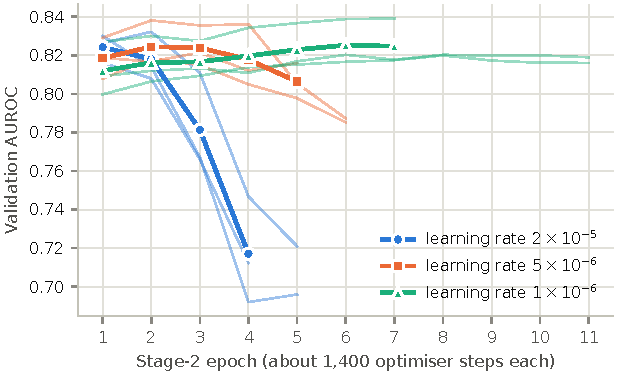
\includegraphics[width=0.62\textwidth]{figures/fig_stage2}
\caption{Validation AUROC during stage-2 fine-tuning for three learning rates. Thin lines are individual seeds and thick lines their mean over the epochs completed by all three seeds. Training stops three epochs after the best validation Challenge score.}
\label{fig:stage2}
\end{figure}

\begin{table}
\caption{Effect of the stage-2 learning rate on configuration B0 (three seeds, mean $\pm$ standard deviation). The ensemble column is the score of the average of the three models.}
\centering
\small
\begin{tabular}{l c c c c c c}
\hline
Stage-2 & \multicolumn{2}{c}{Pooled (A)} & \multicolumn{3}{c}{Within 7.34 s (S7)} & Best stage-2 \\
learning rate & TPR@5\% & AUROC & TPR@5\% & AUROC & Ensemble TPR@5\% & epoch \\
\hline
$2\times10^{-5}$ & $0.436 \pm 0.010$ & 0.829 & $0.384 \pm 0.017$ & 0.787 & 0.404 & 1.7 \\
$5\times10^{-6}$ & $0.423 \pm 0.002$ & 0.834 & $0.381 \pm 0.006$ & 0.792 & 0.396 & 2.7 \\
$1\times10^{-6}$ & $0.404 \pm 0.004$ & 0.830 & $0.362 \pm 0.008$ & 0.784 & 0.375 & 6.7 \\
\hline
\end{tabular}

\label{tab:lr}
\end{table}

\subsection{Removing the cue}
Table \ref{tab:round2} and figure \ref{fig:round2} give the results of the three remedies. Length-matched sampling reduced the length-cue gap from \bzGap{} to \mOneGap, fixed windows reduced it to \wOneGap, and the two together to \mwGap{} (figure \ref{fig:shortcut}(b)). The residual gap with fixed windows alone shows that some of the cue survives when the network cannot see the record length, which is consistent with a difference between the recording devices behind the two formats.

As expected, removing the cue lowered the pooled score: \tpr{} on view A fell from \bzA{} to \mOneA{} with matched sampling and to \mwA{} with both changes. Within short records the scores changed little. The difference from B0 in \tpr{} was \mOneDSseven{} $\pm$ \mOneDSsevenSe{} with matched sampling, \wOneDSseven{} $\pm$ \wOneDSsevenSe{} with fixed windows and \mwDSseven{} $\pm$ \mwDSsevenSe{} with both, and the AUROC rose slightly with fixed windows (\wOneDSsevenAuc{} $\pm$ \wOneDSsevenAucSe; \mwDSsevenAuc{} $\pm$ \mwDSsevenAucSe{} with both). No configuration met the criterion fixed in advance for the primary view.

On records in the 10 s format the picture was different. The AUROC on S10+ rose from \bzStenPlusAuc{} for B0 to \mOneStenPlusAuc{} with matched sampling, \wOneStenPlusAuc{} with fixed windows and \mwStenPlusAuc{} with both (differences from B0 of \mOneDStenPlusAuc{} $\pm$ \mOneDStenPlusAucSe, \wOneDStenPlusAuc{} $\pm$ \wOneDStenPlusAucSe{} and \mwDStenPlusAuc{} $\pm$ \mwDStenPlusAucSe). On S10 alone the AUROC rose from \bzStenAuc{} to \mwStenAuc. The Challenge score on S10+ did not change significantly (\bzStenPlus{} for B0 and \mwStenPlus{} with both changes). The spread between seeds in S7 \tpr{} was smaller with the remedies: a standard deviation of \bzSsevenSd{} for B0 against \mOneSsevenSd, \wOneSsevenSd{} and \mwSsevenSd.

With the cue controlled, fine-tuning the encoder was clearly beneficial. In the combined configuration the frozen encoder ($\alpha=0$) scored \frozenSseven{} on S7 and the fine-tuned encoder ($\alpha=1$) \mwSseven, a mean gain of \ftGainSseven{} that was positive in every seed, with AUROC \frozenSsevenAuc{} against \mwSsevenAuc. The interpolated model ($\alpha=0.5$) scored \halfSseven{} with AUROC \halfSsevenAuc. Interpolation therefore offered no clear advantage over full fine-tuning on these views.

\begin{figure}
\centering
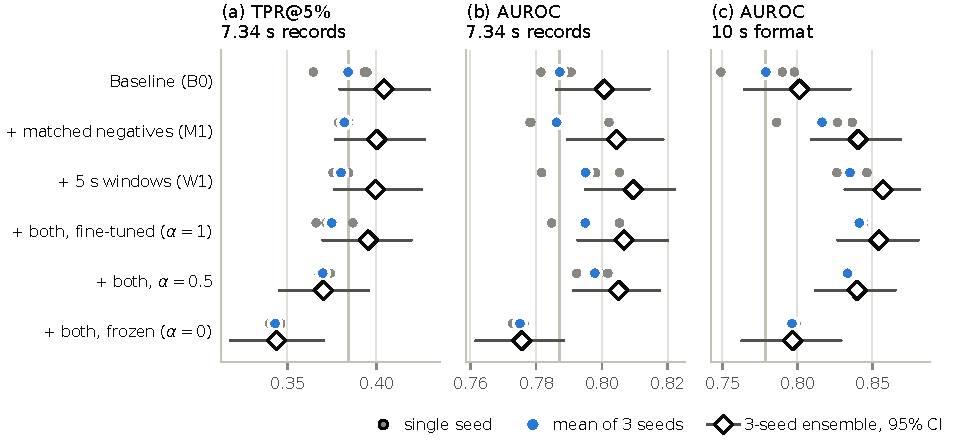
\includegraphics[width=\textwidth]{figures/fig_round2}
\caption{Removing the length cue. Each row is a configuration trained with three seeds. The vertical line marks the mean of the baseline. (a) and (b) use held-out CODE-15\% records of 7.34 s, where neither the source nor the length is informative. (c) uses the 10 s format of the hidden cohorts (view S10+).}
\label{fig:round2}
\end{figure}

\begin{table}
\caption{Results of the remedies (three seeds each). Differences are the mean of the configuration minus the mean of the baseline, with the standard error from a paired bootstrap over test records. The pooled score is \tpr{} on view A.}
\centering
\resizebox{\textwidth}{!}{\begin{tabular}{l c c c c c c c c}
\hline
 & Pooled & \multicolumn{4}{c}{Within 7.34 s records (S7)} & \multicolumn{2}{c}{10 s format (S10+)} & Length- \\
Configuration & TPR@5\% & TPR@5\% & $\Delta$ & AUROC & $\Delta$ & AUROC & $\Delta$ & cue gap \\
\hline
Baseline (B0) & 0.436 & 0.384 & -- & 0.787 & -- & 0.779 & -- & $+0.17$ \\
+ matched negatives (M1) & 0.401 & 0.382 & $-0.002 \pm 0.005$ & 0.786 & $-0.001 \pm 0.003$ & 0.817 & $+0.037 \pm 0.009$ & $+0.04$ \\
+ 5 s windows (W1) & 0.428 & 0.380 & $-0.004 \pm 0.004$ & 0.795 & $+0.008 \pm 0.002$ & 0.835 & $+0.056 \pm 0.010$ & $+0.10$ \\
+ both, fine-tuned ($\alpha=1$) & 0.403 & 0.375 & $-0.009 \pm 0.005$ & 0.795 & $+0.008 \pm 0.003$ & 0.841 & $+0.062 \pm 0.011$ & $+0.01$ \\
+ both, $\alpha=0.5$ & 0.383 & 0.370 & $-0.014 \pm 0.007$ & 0.798 & $+0.011 \pm 0.004$ & 0.833 & $+0.054 \pm 0.012$ & $+0.01$ \\
+ both, frozen ($\alpha=0$) & 0.354 & 0.343 & $-0.041 \pm 0.009$ & 0.775 & $-0.012 \pm 0.006$ & 0.797 & $+0.017 \pm 0.017$ & $+0.00$ \\
\hline
\end{tabular}
}
\label{tab:round2}
\end{table}

\begin{figure}
\centering
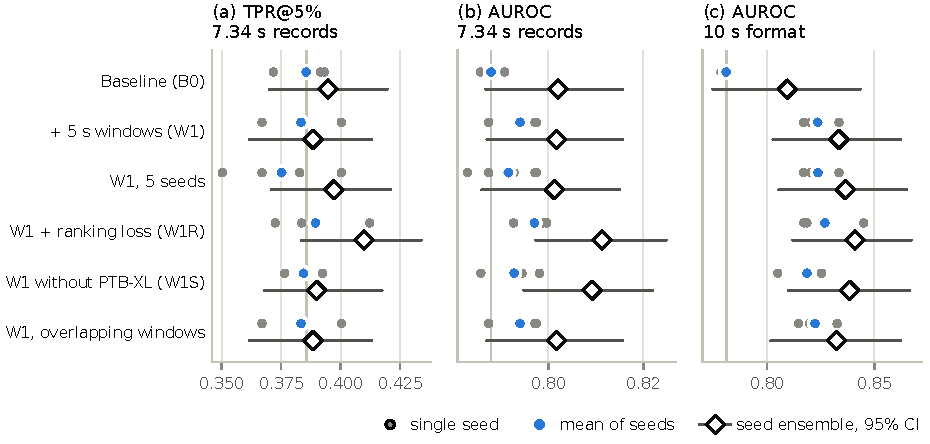
\includegraphics[width=\textwidth]{figures/fig_round3}
\caption{Round 3 under the fixed validation protocol. Each row is a configuration trained with three seeds (five for the row so labelled). The vertical line marks the mean of the baseline. (a) and (b) use held-out CODE-15\% records of 7.34 s; (c) uses the 10 s format of the hidden cohorts (view S10+).}
\label{fig:round3}
\end{figure}

\begin{table}
\caption{Round 3 (fixed validation protocol; three seeds each unless stated). Differences are the mean of the configuration minus the mean of the baseline, with the standard error from a paired bootstrap over test records. The length-cue gap is the mean predicted probability of short CODE-15\% negatives minus that of long ones; the source gap is the mean probability of SaMi-Trop positives minus that of CODE-15\% positives.}
\centering
\resizebox{\textwidth}{!}{\begin{tabular}{l c c c c c c c c c c}
\hline
 & Pooled & \multicolumn{4}{c}{Within 7.34 s records (S7)} & \multicolumn{3}{c}{10 s format (S10+) AUROC} & Length- & Source \\
Configuration & TPR@5\% & TPR@5\% & $\Delta$ & AUROC & $\Delta$ & mean & $\Delta$ & ensemble & cue gap & gap \\
\hline
Baseline (B0) & 0.427 & 0.385 & -- & 0.788 & -- & 0.781 & -- & 0.809 & $+0.15$ & $-0.04$ \\
+ 5 s windows (W1) & 0.422 & 0.383 & $-0.002 \pm 0.005$ & 0.794 & $+0.006 \pm 0.002$ & 0.824 & $+0.043 \pm 0.010$ & 0.834 & $+0.08$ & $-0.02$ \\
\quad W1 with 5 seeds & 0.417 & 0.375 & $-0.010 \pm 0.005$ & 0.792 & $+0.004 \pm 0.002$ & 0.824 & $+0.043 \pm 0.010$ & 0.837 & $+0.08$ & $-0.02$ \\
W1 + ranking loss (W1R) & 0.425 & 0.389 & $+0.004 \pm 0.005$ & 0.797 & $+0.009 \pm 0.003$ & 0.827 & $+0.046 \pm 0.012$ & 0.841 & $+0.01$ & $-0.01$ \\
W1 without PTB-XL (W1S) & 0.414 & 0.384 & $-0.001 \pm 0.005$ & 0.793 & $+0.005 \pm 0.003$ & 0.819 & $+0.038 \pm 0.011$ & 0.839 & $+0.07$ & $-0.01$ \\
\quad W1, windows every 2.5 s & 0.422 & 0.383 & $-0.002 \pm 0.005$ & 0.794 & $+0.006 \pm 0.002$ & 0.822 & $+0.041 \pm 0.010$ & 0.832 & $+0.09$ & $-0.02$ \\
\hline
\end{tabular}
}
\label{tab:round3}
\end{table}

\subsection{Seed ensembles and perturbations}
Averaging three seeds improved the baseline from \bzA{} to \bzEnsA{} in \tpr{} on view A and from \bzSseven{} to \bzEnsSseven{} within short records, where the AUROC rose from \bzSsevenAuc{} to \bzEnsSsevenAuc. The ensemble of the combined configuration scored \mwEnsSseven{} on S7 and reached an AUROC of \mwEnsStenPlusAuc{} on S10+, against \bzEnsStenPlusAuc{} for the baseline ensemble. On the primary view, no modelling change in this study produced a gain as large as that of ensembling.

The perturbations of view C had little effect once the comparison was made within length groups: \tpr{} within short records was \bzSsevenC{} for B0 and \mwSsevenC{} for the combined configuration on the perturbed records, close to the unperturbed values.

\subsection{Round 3: the candidate under the fixed validation protocol}
\label{sec:res-r3}
Table \ref{tab:round3} and figure \ref{fig:round3} give the results. Under the fixed protocol the baseline scored \rThreeBzSseven{} within short records and \rThreeBzStenPlusAuc{} AUROC on the 10 s format, close to its round-2 values, so the protocol itself changed little. The fixed-window model again left the S7 score unchanged (\rThreeWoneDSseven) and raised the S10+ AUROC by \rThreeWoneDStenPlusAuc, and this time it met the rule, which had been written for the 10 s format. The ranking loss (W1R) and the removal of PTB-XL (W1S) also passed against the baseline (S10+ AUROC \rThreeWoneRDStenPlusAuc{} and \rThreeWoneSDStenPlusAuc), as did overlapping windows (\rThreeWoneTtaDStenPlusAuc). Against W1, which was the candidate carried in, none of them gained on the primary metric by more than one SE (W1R \rThreeWoneRVsWoneDStenPlusAuc, W1S \rThreeWoneSVsWoneDStenPlusAuc, overlapping windows \rThreeWoneTtaVsWoneDStenPlusAuc). On the S7 score the ranking loss gained \rThreeWoneRVsWoneDSseven{} over W1, just over one SE, without losing on S10+, which is the secondary criterion of the rule; W1S (\rThreeWoneSVsWoneDSseven) did not, and overlapping windows cannot change S7 at all, because for a 7.34 s record the two placements give the same two windows. Applied as written, the rule therefore made W1R the entry. We note that the margin is small and that the criterion was met by one SE, not by the two or three that would make it convincing on its own. The ranking loss had one clear effect: it reduced the length-cue gap from \rThreeWoneGap{} to \rThreeWoneRGap, so the network stopped scoring the padded 7.34 s negatives above the 10.24 s ones even though it could not see the record length, and its three-seed ensemble reached \rThreeWoneREnsSseven{} on S7 (\rThreeWoneRVsWoneDEnsSseven{} against the W1 ensemble) and \rThreeWoneREnsStenPlusAuc{} AUROC on S10+, the highest ensemble values of the study. The source gap, the mean probability of SaMi-Trop positives minus that of CODE-15\% positives, was \rThreeBzSrcGap{} for the baseline and \rThreeWoneSSrcGap{} without PTB-XL, so removing the European negatives did not make the positives more separable by source. The five-seed ensemble of W1 scored \rThreeWfiveEnsStenPlusAuc{} on S10+ against \rThreeWoneEnsStenPlusAuc{} for three seeds (\rThreeWfiveVsWoneDEnsStenPlusAuc), inside one SE, so three members suffice.

\section{Discussion}
\subsection{A shortcut inside the largest training source}
The length of a CODE-15\% recording is a strong predictor of its Chagas label: used alone, it reaches an AUROC of \durOnlyB{} among CODE-15\% records. We do not know the cause. The two lengths are likely to correspond to two recording systems or software versions in the telehealth network that collected the data \citep{ribeiro2020}, deployed in regions or periods with different prevalence of Chagas disease. This would also explain why a model that cannot observe the record length still separates the two formats to some extent, since devices differ in filtering and noise. We could not test this explanation, because the public data carry no device or site information.

Whatever its origin, the association cannot help on the hidden cohorts, whose recordings are all about 10 s long \citep{reyna2025}. It is a plausible contributor to the gap between internal and hidden scores that almost every team observed. Two of the three highest-ranked entries used augmentations that blur the cue. The winning team cropped records at random to between 5.65 and 10 s and zero-padded them \citep{vansantvliet2025}, and the third-placed team masked the beginning and end of records ``to simulate shorter signals'' \citep{hong2025}. Both make the amount of padding less informative, although neither team described the association with the label. In our own Challenge paper we listed random padding or windowing as untested future work \citep{nguyen2025}.

\subsection{What the ablation did and did not show}
The ablation illustrates how such a cue can mislead model development. On the pooled held-out set the final model scored \ladderGainA{} higher than the entry, and four of the eight steps raised the score. Within records of equal length the improvement disappeared. Fine-tuning the encoder while it received age and sex lowered the mean predicted probability of the PTB-XL records, which are all negative, from \ptbRowFour{} to \ptbRowFive. This is the signature of a model becoming better at recognising where a record came from. Removing age and sex brought the value back to \ptbRowFiveB{} with no loss of performance, which is why the final configuration does not use them. A patient-grouped split and natural prevalence, both of which we consider necessary, did not protect against this.

Several of our expectations were refuted, and we report them because the pre-specified rules make the negative results informative. A lower stage-2 learning rate did not help. Using all negatives was worse than using a third of them. Interpolating between the frozen and fine-tuned weights did not beat full fine-tuning. Once the length cue was controlled, fine-tuning the encoder gave a clear within-length gain over a frozen encoder, in contrast to what the pooled ablation had suggested. Finally, the remedies did not improve the primary view. They removed the cue and improved the AUROC in the 10 s format by several standard errors, but by the rule we set in advance they did not earn adoption on within-short performance alone. We report this as it stands. Because the hidden cohorts are 10 s recordings, the final round made the 10 s format the primary view, a change recorded with its reason before the runs, and under a validation protocol that cannot reward the shortcut the fixed-window model with the hard-negative ranking loss was adopted as the entry; the 10 s result remains a hypothesis until it is scored on the hidden cohorts.

\subsection{Recommendations}
For work on these data we suggest the following.
\begin{enumerate}
\item Report performance within recording formats. For CODE-15\% this means scoring 7.34 s and 10.24 s records separately. The duration-only baseline and the length-cue gap are cheap checks of whether a model depends on length.
\item Remove the cue at the data level. Sampling negatives to match the length distribution of the positives is free when negatives are abundant, and a fixed window that never requires padding makes the length invisible to the network.
\item Expect pooled internal scores to fall when a shortcut is removed, and decide in advance which views are decision metrics.
\item Average several seeds. It was the most reliable improvement we found and it reduces the noise that otherwise dominates comparisons of single runs.
\end{enumerate}

\subsection{Limitations}
We could not score models on the hidden cohorts after the Challenge closed, so the claim that removing the length cue improves external performance remains untested. The 10.24 s group of our held-out set has only \nStenPos{} CODE-15\% positives, and the larger view S10+ includes SaMi-Trop positives, which may be recognisable by their source. All results come from one held-out split and one backbone. The ablation steps before B0 were single runs, although the final comparisons used three seeds. CODE-15\% labels are self-reported, which limits what any internal evaluation can show. The attribution of the length association to recording devices is a hypothesis. The round-3 rule was set after round 2 had shown the 10 s-format gain; it was fixed before the round-3 runs and applied to a re-trained baseline, but it was informed by the earlier result.

\section{Conclusion}
In the public training data of the PhysioNet Challenge 2025, the length of a CODE-15\% recording is a strong predictor of its Chagas label and is absent from the hidden cohorts. Models trained on these data use it, pooled internal metrics reward it, and a careful-looking ablation can be driven by it. Scoring within recording formats exposes the problem, and length-matched sampling with fixed-length windows removes the cue with little change in within-format performance and a higher AUROC on recordings in the format of the hidden cohorts. With validation carved before the negative cap, independent of the seed and scored within the shortcut-free format, a three-seed ensemble of the fixed-window model with a hard-negative ranking loss is our entry for external evaluation.

\ack{% TODO(authors): edit as appropriate.
The authors thank the organisers of the George B. Moody PhysioNet Challenge 2025 and the teams whose published methods informed this study.
% TODO(authors): IOP Publishing requires disclosure of generative AI use; confirm or rewrite the next two sentences.
An AI coding assistant (Claude, Anthropic) was used under the authors' direction to implement and run the experiments, analyse the results and draft this manuscript. The authors reviewed the code, results and text and take responsibility for the content.}

\funding{% TODO(authors): funding statement.
To be completed by the authors.}

\roles{% TODO(authors): CRediT author contributions.
To be completed by the authors.}

\data{The CODE-15\%, SaMi-Trop and PTB-XL data are publicly available through the Challenge \citep{reyna2025}. The code, the configuration of every run, the record-length table and the scripts that generate each figure, table and number in this paper are in the project repository (to be made public by the authors).}

\bibliographystyle{plainnat}
\bibliography{refs}
\end{document}
